\section{Summary}

Checking conflict-serializability would be efficient if the conflict graph were known from the outset, but in practice, it is typically not.
Therefore, a scheduler must work online. 
It is impractical to maintain, update, and check the conflict graph at each operation request. 
Additionally, the assumption that concurrency control can rely solely on the commit-projection of the schedule is unrealistic because aborts do occur.
Thus, an online scheduler needs a simple decision criterion that avoids as many anomalies as possible with minimal overhead.

\paragraph*{Online concurrency control}
In the realm of online concurrency control, considering arrival sequences is crucial.
The concurrency control system translates an arrival sequence into an effective a posteriori schedule.
Two main families of techniques are commonly employed for online scheduling:
\begin{itemize}
    \item Pessimistic techniques (\textit{locks}): if a resource is taken, make the requester wait or pre-empt the holder.
    \item Optimistic techniques (\textit{timestamps}): serve as many requests as possible, possibly using out-of-date versions of the data. 
\end{itemize}
In practice, commercial systems often combine elements from both pessimistic and optimistic approaches to leverage the strengths of each.

\subsection{Isolation levels in SQL '99}
SQL defines transaction isolation levels that specify the anomalies to be prevented when running at each level:

\begin{table}[H]
    \centering      
    \begin{tabular}{c|ccc|}
    \cline{2-4}
                                                    & \textbf{Dirty read} & \textbf{Non-repeatable read} & \textbf{Phantoms}    \\ \hline
    \multicolumn{1}{|c|}{\textbf{Read uncommitted}} & $\checkmark$        & $\checkmark$                 & $\checkmark$         \\
    \multicolumn{1}{|c|}{\textbf{Read committed}}   & $\tikzxmark$        & $\checkmark$                 & $\checkmark$         \\
    \multicolumn{1}{|c|}{\textbf{Repeatable reads}}  & $\tikzxmark$        & $\tikzxmark$                 & $\checkmark$(insert) \\
    \multicolumn{1}{|c|}{\textbf{Serializable}}     & $\tikzxmark$        & $\tikzxmark$                 & $\tikzxmark$         \\ \hline
    \end{tabular}
\end{table}
The four levels are implemented respectively with: no read locks, normal read locks, strict read locks, and strict locks with predicate locks. 
\texttt{Serializable} is not the default because its strictness can lead to the following problems:
\begin{itemize}
    \item Deadlock: two or more transactions are in endless mutual wait. 
    \item Starvation: a single transaction is in endless wait. 
\end{itemize}

\subsection{Concurrency classes sets}

Here is the final configuration for the sets of concurrency classes: 
\begin{figure}[H]
    \centering
    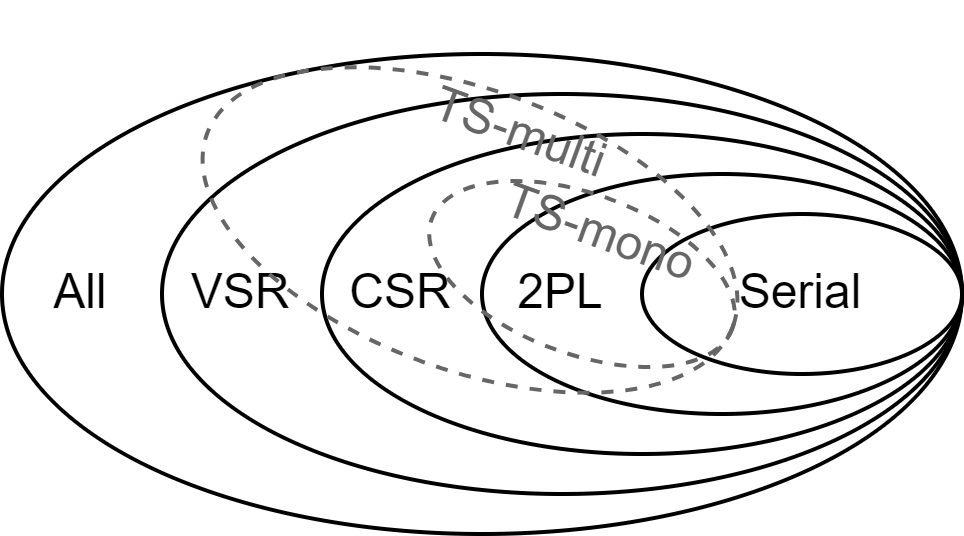
\includegraphics[width=0.65\linewidth]{images/set.png}
\end{figure}